\chapter{Tree width}

\section{Dynamisches Programm für Vertex Cover}
  \marginpar{3.7.12}
  
  Zunächst betrachten wir Vertex Cover auf Bäumen. Dazu berechnen wir, beginnend bei den Blättern, für jeden Teilbaum mit Wurzel \(v\) ein ein maximales Vertex Cover, in dem \(v\) enthalten ist, und ein Vertex Cover, in dem die Teilbaum-Wurzel \(v\) nicht enthalten ist. Wir speichern die Ergebnisse der Berechnung in den Tabellen \(IN(v)\) bzw. \(OUT(v)\) für Teilbäume mit Wurzel \(v\), in denen \(v\) enthalten bzw. nicht enthalten ist.

  Zur Berechnung von \(OUT(v)\) für einen beliebigen Knoten \(v\) berechnen wir (in binären Bäumen) \(IN(v_1) + IN(v_2)\) der beiden Kind-Knoten \(v_1\) und \(v_2\) von \(v\). Wir müssen \(v_1\) und \(v_2\) in das Vertex Cover aufnehmen, da die Kanten \((vv_1)\) und \((vv_2)\) gecovert werden müssen.

  Zur Berechnung von \(IN(v)\) berechnen wir \(\max \{ IN(v_1), OUT(v_2) \} + \max \{ IN(v_2), OUT(v_2) \}\), da die Kanten \((vv_1)\) und \((vv_2)\) bereits durch \(v\) gecovert sind und wir daher die Wahl haben, ob wir \(v_1\) bzw. \(v_2\) in das Vertex Cover aufnehmen.

  Diese Berechnung kann in \(O(\deg v)\) Zeit durchgeführt werden, wenn die Werte \(IN(v_1), ..., IN(v_{\deg v})\) und \(OUT(v_1), ..., OUT(v_{\deg v})\) bereits bekannt sind. Für alle Knoten ausgeführt, erhält man \(O(n)\), denn die Anzahl von Kanten im Baum beträgt \(n-1\).

\section{Definition}
  
  Sei \(G = (V,E)\) ein Graph. Eine \defNotion{tree decomposition} von \(G\) ist ein Paar \(\tdc{T} = ( \{ X_i : i \in I \}, T )\), wobei jedes \(X_i\) Teilmengen von \(V\) sind, die man \defNotion{bags} nennt, und \(T\) ein Baum mit der Knotenmenge \(I\) ist. Außerdem müssen noch weitere Eigenschaften gelten:
  \begin{enumerate}[(i)]
   \item Es gilt \(\bigcup_{i \in I} X_i = V\).
   \item Für jede Kante \((uv) \in E\) gibt es ein \(i \in I\) mit \(\{u,v\} \subseteq X_i\).
   \item Für alle \(i,j,k \in I\) so dass \(j\) auf einem Pfad zwischen \(i\) und \(k\) in \(T\) liegt, gilt \(X_i \cap X_k \subseteq X_j\).
  \end{enumerate}
  
  Die \defNotion{width} einer \defNotion{tree decomposition} wird definiert als \(\max \{ |X_i| : i \in I \} - 1\). Die \defNotion{tree width} \(\tw(G)\) eines Graphen \(G\) ist die kleinste natürliche Zahl \(w\), für die eine tree decomposition mit width \(w\) existiert.

\section{Beispiele}

  \begin{figure}[H]
    \centerline{
      \xymatrix{
        &&& 1 \\
        && 2 \ar@{-}[ur] \\
        & 3 \ar@{-}[ur] && \ar@{-}[ul] 4 \\
        5 \ar@{-}[ur] && 6 \ar@{-}[ul] \\
      }
    }
    \caption{Beispiel (a): Eine tree decomposition dieses Graphen ist \(G\) selbst, wobei jedes bag zwei Knoten enthält. Die Menge der bags ist dann \( \{ \{1,2\}, \{2,3\}, \{2,4\}, \{3,5\}, \{3, 6\} \} \).}
  \end{figure}

  \begin{figure}[H]
    \centerline{
      \xymatrix{
        && \{ 1,2 \} \\
        & \{2,3\} \ar@{-}[ur] && \ar@{-}[ul] \{ 2,4 \} \\
        \{3,5\} \ar@{-}[ur] && \{3,6\} \ar@{-}[ul]
      }
    }
    \caption{Die bags der tree decomposition aus \(G\) wie oben definiert.}
  \end{figure}

  Wie im Beispiel gesehen, haben alle Bäume stets tree width 1. Als nächstes Beispiel (b) betrachten wir einen Kreis mit \(n\) Knoten.

  \begin{figure}[H]
    \centerline{
      \xymatrix{
        && \circ \ar@{-}[r] & \circ & \\
        &\circ \ar@{-}[ur] &&& \circ \ar@{-}[ul] \\
        &\circ \ar@{-}[u] &&& \circ \ar@{-}[u] \\
        && \circ \ar@{-}[ul] \ar@{-}[r] & \circ \ar@{-}[ur] & \\
        \circ \ar@{-}[r] & \circ \ar@{-}[r] & \circ \ar@{-}[r] & \circ \ar@{-}[r] & \circ \ar@{-}[r] & \circ \ar@{-}[rd] \\
        & \circ \ar@{-}[lu] & \circ \ar@{-}[l] & \circ \ar@{-}[l] & \circ \ar@{-}[l] & \circ \ar@{-}[l] & \circ \ar@{-}[l] \\
      }
    }
    \caption{Beispiel (b): Zwei Bilder des selben Graphen \(C_n\). Als bags wählt man die Mengen aus den drei linken und drei rechten Knoten, sowie jeweils 3 nebeneinanderliegende Knoten sowie einen gegenüberliegenden.}
  \end{figure}

  \begin{figure}[H]
    \centerline{
      \xymatrix{
        \circ \ar@{-}[r] & \circ && \circ \ar@{-}[r] \ar@{-}[rd] & \circ \\
        \circ &&&& \circ
      }
    }
    \caption{Bags der tree decomposition im Kreis \(C_n\), also tree width 2.}
  \end{figure}  

  \begin{figure}[H]
    \centerline{
      \xymatrix{
        \circ \ar@{-}[r] \ar@{-}[d] & \circ \ar@{-}[r] \ar@{-}[d] & \circ \ar@{-}[r] \ar@{-}[d] & \circ \ar@{-}[r] \ar@{-}[d] & \circ \ar@{-}[r] \ar@{-}[d] & \circ       \ar@{-}[d] \\
        \circ \ar@{-}[r]        & \circ \ar@{-}[r]        & \circ \ar@{-}[r]        & \circ \ar@{-}[r]        & \circ \ar@{-}[r]        & \circ
      }
    }
    \caption{Beispiel (c): Eine Leiter \(G\), die bags der tree decomposition sind wiederum 3-Mengen aus "`L"' wie beim Kreis \(C_n\)}
  \end{figure}

  \begin{figure}[H]
    \centerline{
      \xymatrix{
        \circ \ar@{-}[r] \ar@{-}[d] & \circ \ar@{-}[r] \ar@{-}[d] & \circ \ar@{-}[d] \ar@{-}[r] & \circ \ar@{-}[r] \ar@{-}[d] & \circ \ar@{-}[r] \ar@{-}[d] & \circ       \ar@{-}[d] \\
        \circ \ar@{-}[r]        & \circ \ar@{-}[r] \ar@{-}[d] & \circ \ar@{-}[d] \ar@{-}[r] & \circ \ar@{-}[r]        & \circ \ar@{-}[r]        & \circ \\
                            & \circ \ar@{-}[r] \ar@{-}[d] & \circ \ar@{-}[d] \\
                            & \circ \ar@{-}[r] \ar@{-}[d] & \circ \ar@{-}[d] \\
        \circ \ar@{-}[r] \ar@{-}[d] & \circ \ar@{-}[r] \ar@{-}[d] & \circ \ar@{-}[d] \ar@{-}[r] & \circ \ar@{-}[r] \ar@{-}[d] & \circ \ar@{-}[d] \\
        \circ \ar@{-}[r]        & \circ \ar@{-}[r] \ar@{-}[d] & \circ \ar@{-}[d] \ar@{-}[r] & \circ \ar@{-}[r]        & \circ \\
                            & \circ \ar@{-}[r]        & \circ  \\
      }
    }
    \caption{Beispiel (c'): Eine modifizierte Leiter \(G\), die bags der tree decomposition sind 4-Mengen aus benachbarten Knoten (quadratisch angeordnet)}
  \end{figure}

  Beispiel (d): Der vollständige Graph \(K_n\). Seine tree width beträgt \(n-1\), da alle Knoten in ein bag der tree decomposition müssen.

  Beispiel (e): Ein Gitter-Graph \(G\) mit \(k \cdot l\) Knoten. Als Bags wählen wir jeweils zwei benachbarte Spalten, damit erhalten wir eine obere Schranke von \(\tw(G) \leq 2 \cdot \min \{ k,l \}\).

  \marginpar{17.7.12}
  
  \begin{figure}[H]
    \centerline{
      \xymatrix{
          & c &   &   & h \ar@{-}[rd] \\
        b \ar@{-}[ru] \ar@{-}[rr] \ar@{-}[d] \ar@{-}[drr] &   & d \ar@{-}[lu] \ar@{-}[rru] &   &   & i \\
        a \ar@{-}[rru] &   & \ar@{-}[u] e \ar@{-}[rruu] \ar@{-}[rr] &   & g \ar@{-}[uu] \\
          &   &   & f \ar@{-}[ru] \ar@{-}[lu]
      }
    }
    \caption{Beispiel (f)}
  \end{figure}

  \begin{figure}[H]
    \centerline{
      \xymatrix{
        & & deh & \ar@{-}[l] ih \\
        bcd \ar@{-}[r] & bde \ar@{-}[ur] & egh \ar@{-}[u] \\
        & abd \ar@{-}[u] & efg \ar@{-}[u]
      }
    }
    \caption{Tree decomposition für Beispiel (f)}
  \end{figure}
  
  \begin{theorem}
    Planare Graphen haben tree width \(O(\sqrt{n})\).
  \end{theorem}

  \begin{theorem}
    Eine tree decomposition der width \(k\) eines Graphen \(G\) mit tree width kleiner oder gleich \(k\) kann in \(2^{O(k^3)} \cdot n\) Zeit berechnet werden.
  \end{theorem}

\section{Verbessertes dynamisches Programm für Vertex Cover für Graphen mit beschränkter Tree Width}
  
  \begin{theorem}
    Für einen Graphen \(G\) mit einer tree decomposition \(\widetilde{T} = ( \{ X_i : i \in I \}, T) \) mit width \(k\) kann ein optimales vertex cover in \(O(2^k k |I|)\) Zeit berechnet werden.
  \end{theorem}

  Wir verwenden die folgende Idee. Für jeden bag \(X_i\) überprüfen wir für alle \(2^{|X_i|}\) Möglichkeiten, ob diese ein Vertex Cover für \(G[X_i]\) darstellen. Diese Information speichern wir in der Tabelle \(A_i\). Das optimale Vertex Cover berechnen wir dann mit einem bottom-up dynamischen Programm in \(\widetilde{T}\). Die Schwierigkeit dabei ist die Sicherstellung der Konsistenz durch das Aktualisieren der Tabelle beim Verarbeiten der Kanten. Dazu verwenden wir folgende Schritte:

  \begin{enumerate}
   \setcounter{enumi}{-1}
   \item \textbf{table creation.} Für jeden bag \(X_i = \{ x_{i1}, ..., x_{in} \}, n_i = |X_i|\) legen wir eine Tabelle \(A_i\) folgender Form mit \(2^{k_i}\) Zeilen an:
   
      \begin{center}\begin{tabular}{cccc|c}
        \(x_{i1}\) & \(x_{i2}\) & \(\cdots\) & \(x_{i_{n_i}}\) & \(m_i\) \\ \hline
        0 & 0 & \(\cdots\) & 0 \\
        0 & 0 & \(\cdots\) & 1 \\
        \(\vdots\) &  &  & \(\vdots\) \\
        1 & 1 & \(\cdots\) & 1 \\
      \end{tabular}\end{center}

      Eine \defNotion{Zuordnung} für ein bag \(X_i\) ist eine Abbildung \(C_i : X_i \to \{0,1\}\), die für jeden Knoten in \(X_i\) festlegt, ob er im Vertex Cover enthalten ist. Die Tabelle \(A_i\) hat eine Zeile für jede mögliche Zuordnung von \(X_i\). Wir setzen nun \(V_i := \bigcup_{j \in T_i} X_i\). Ziel ist es, für jede Zuordnung \(C_i\) von \(X_i\) den Wert
      \[m_i(C_i) := \min \{ |V'| : V' \subseteq V_i \text{ ist ein Vertex Cover für \(G[V_i]\) das \(C_i\) respektiert} \} \]
      berechnen. \(C_i\) \defNotion{wird von \(V'\) respektiert}, wenn \(V' \cap V_i = C_i^{-1}(1)\) gilt.

      \begin{figure}[h]
        \centering
        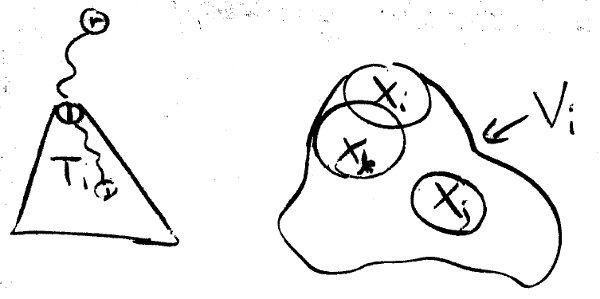
\includegraphics[width=.5\textwidth]{./Bilder/b04.jpg}
        % b04.jpg: 600x299 pixel, 72dpi, 21.17x10.55 cm, bb=0 0 600 299
        \caption{Skizze zum Vorgehen bei der Berechnung des Vertex Cover durch ein dynamisches Programm}
      \end{figure}

    \item \textbf{table init.} Sei \(X_i\) ein bag und \(C_i\) eine Zuordnung für \(X_i\). Wir nennen \(C_i\) genau dann \defNotion{gültig}, wenn \(C_i{-1}(1)\) ein Vertex Cover für \(G[X_i]\) ist. Wir initialisieren für jede Zuordnung \(C_i\) den Wert \(m_i\) nach der Vorschrift
    \[
     m_i(C_i) :=
     \begin{cases}
       |C_i^{-1}(1)| & (C_i \text{ ist gültig}), \\
       \infty & (\text{sonst}).
     \end{cases}
    \]

    \item \textbf{dynamic program.} Wir durchlaufen den Baum bottom-up und aktualisieren "`adjazente"' Tabellen gegeneinander. Sei \(i \in I\) der Vater von \(j \in I\). Wir nehmen weiterhin an, dass
    \begin{eqnarray*}
      X_i &=& \{ z_1, ..., z_s, v_1, ..., v_{t_i} \}, \\
      X_j &=& \{ z_1, ..., z_s, u_1, ..., u_{t_j} \}. 
    \end{eqnarray*}
    Es folgt unmittelbar \(X_i \cap X_j = \{ z_1, ..., z_s \}\). Eine \defNotion{Erweiterung} einer Zuordnung \(C : W \to \{0,1\}\) ist eine Zuordnung \(\widetilde{C} : \widetilde{W} \to \{0,1\}\) mit \(\widetilde{W} \supseteq W\) und \(\widetilde{C}|_W = C\).

    Für jede Zuordnung \(C : \{ z_1, ..., z_s \} \to \{0,1\}\) und jede Erweiterung \(C_i : X_i \to \{0,1\}\) aktualisieren wir gemäß
    \[
      m_i(C_i) := m_i(C_i) + \min \{ m_j(C_j) : C_j : X_j \to \{0,1\} \text{ ist Erweiterung von } C \} - | C^{-1}(1) |.
    \]
    Der Term \(| C^{-1}(1) |\) vermeidet Doppelzählungen.

    Hat \(i\) mehrere Kindknoten \(j_1, ..., j_l\) in \(T\), dann wird \(A_i\) für jedes Kind analog aktualisiert. Schritt 2 stoppt, wenn die Wurzel des Baumes erreicht wurde.

  \item \textbf{result.} Die Größte des minimalen Vertex Cover kann aus der Tabelle \(A_r\) der Wurzel des Baumes abgelesen werden, denn es ist gegeben durch
  \[ \min \{ m_r(C_r) : C_r \text{ ist eine Zuordnung für } X_i \}. \]
  Durch Speichern der Vertex Cover der Teilbäume für jede Zurordnung und jeden bag kann man auch das Vertex Cover selbst berechnen.
  \end{enumerate}

  Für die Laufzeitanalyse genügt es zu zeigen, dass die Aktualisierung in \(O(2^kk)\) durchzuführen ist.

